\documentclass[11pt,leqno]{book}
\textwidth 13.5cm
\textheight 18.5cm
\topmargin 0in
\parindent 0.5cm
\oddsidemargin 0.5in
\evensidemargin 0.5in
\usepackage{amssymb}
\usepackage{amsmath}
\usepackage{graphicx,wrapfig,url,rotating,array}
\usepackage{fan}
\usepackage{subcaption}
\usepackage{placeins}

\def\bibname{{\Large\bf References}}
\def\thebibliography#1{\addvspace{3em}\noindent
\noindent \bibname  \list
 {[\arabic{enumi}]}{\settowidth\labelwidth{[#1]}\leftmargin\labelwidth
 \advance\leftmargin\labelsep
 \usecounter{enumi}}
 \def\newblock{\hskip .11em plus .33em minus .07em}
 \sloppy\clubpenalty4000\widowpenalty4000
 \sfcode`\.=1000\relax}
\let\endthebibliography=\endlist

\usepackage[english]{babel}

\pagestyle{fancy}
\footrulewidth 0pt
\headrulewidth 0.5pt
\lfoot[\thepage]{} \cfoot[]{} \rfoot[]{\thepage}
\lhead[Geometric Visualization of a Polygon Area Partitioning]{ESGI'132} \chead[]{} \rhead[ESGI'132]{Geometric Visualization of a Polygon Area Partitioning}

\def\efig#1#2{\includegraphics[width=#2mm]{#1}}
\def\efigsc#1#2{\includegraphics[scale=#2]{#1}}
\def\TTT{\end{document}}
\def\bt{\begin{tabular}}
\def\et{\end{tabular}}
\def\cl{\centerline}
\def\mc{\multicolumn}

\def\diag{\mathop{\rm diag}}
\thispagestyle{empty}
\newcommand{\sect}[1]{\vskip7mm\par{\large \bf #1}}
\newcommand{\subsect}[1]{\vskip 3mm\par{\bf#1}}

 \def\hlst{\setlength{\topsep}{1pt}\setlength{\partopsep}{1pt}%
 \setlength{\parsep}{1pt}\setlength{\itemsep}{\parskip}}

\begin{document}

\begin{center}
\textbf{\LARGE Geometric Visualization of a Polygon Area Partitioning}

\vspace*{5mm}

Todor Balabanov,
Stanislav Darachev,
Ivan Jordanov,
Aleksandar Karakushev,
Nikolai Kitanov,
Alexander Manov,
Georgi Nikolov,
Spasimir Nonev,
Zdravka Nedyalkova,
Emiliyan Rogachev,
Natasha Stojkovikj,
Petar Tomov,
Iliyan Zankinski

\end{center}

\date{18-22 Sep 2017}

\sect{Abstract}

In the process of modeling sewerage networks, the main component is the drained area (catchment) from which water is collected to each conduit (pipe). If the area for a single subcatchment is derived from a mathematical model, we have to create the geometry of that territory. For visualization purpose, we need to find geometric partitioning of the polygon. In this paper solutions for geometric visualization of a polygon partitioning are proposed.

\textit{Key words}: visualization, polygon area partitioning, optimal cutting problem

\sect{1.~Introduction}

In the process of modeling sewerage networks, the main component is the drained area (catchment) from which water is collected to each conduit (pipe). If the area for a single sub-catchment is derived from a mathematical model, we have to create the geometry of that territory. In this paper we want to make geometric visualization for partitioning of a given living area. Partitioning is done according known water debit relative to each pipe. All pipes are associated to with edges of a polygon (single pipe for a single edge). The fianl goal is to generate geometric visualization of a polygon partitioning.  

This problem is very common in hydrology and limited information is published in the hydrological literature. Two approaches for automated generation of Thiessen polygons are considered in \cite{han:bra:1} - triangulation method and grid method. The ways for their implementation in hydrological applications is also given. Description of procedure to derive the relationship between the catchment area, grid size and accuracy indicator based on weighted mean error is also provided. Web-based urban water management modeling platform for simplifying the setup and use of complex integrated models is presented in \cite{mai:mik:1}. The paper demonstrates how flooding behavior of new urban developments can easily be assessed with the web platform, i.e. to inform discussions in interdisciplinary and interactive stakeholder workshops. The workflow of the used DynaMind model is also shown. As input it uses user defined catchments. Catchments are presented as polygons in a sewer system model. The polygon is divided into several smaller polygons (sub-catchments) Gaussian distributed. New inlet nodes within the polygon and creating a Voronoi diagram on the bases of these nodes. Generation of three dimensional models of large urban/suburban environments is described in \cite{lay:day:1}. Automated tools are used to provide a rapid coarse model of a city. These techniques are tailored to generate geometry of appropriate complexity for real-time rendering, thereby negating the need for the simplification stage. Roof modelling for rectilinear polygons is used and procedure for partitioning of a polygon into rectangles is described. Paper \cite{lockie:1} outlines the technical capability and functionality of Storm Water Management Model (SWMM). Also the advantages, disadvantage and applicability of SWMM are discussed and a brief comparison between SWMM and other common hydraulic models is presented. The hydraulic engine of SWMM has been proven and tested more than 40 years and is reported as the most widely applied stormwater model in United States and New Zealand.

\begin{figure}[h!]
\centering
\begin{subfigure}{.5\textwidth}
  \centering
  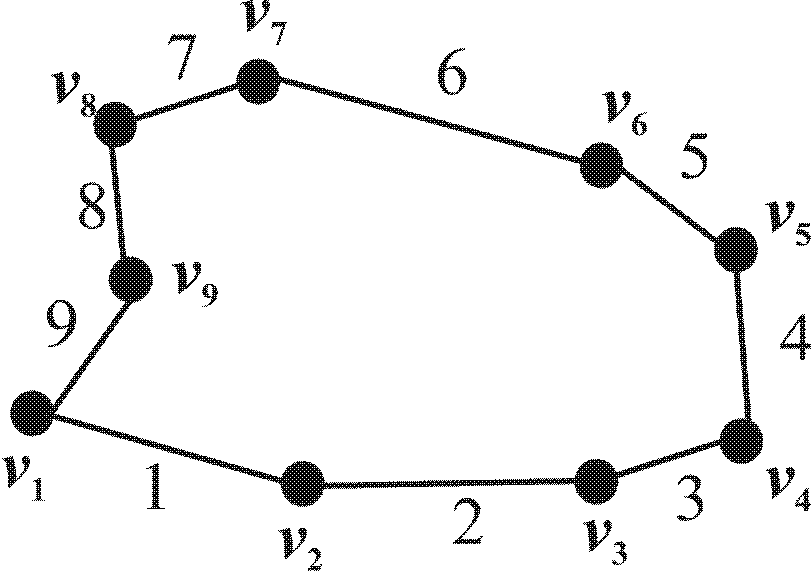
\includegraphics[width=.5\linewidth]{pic01.png}
  \caption{Input polygon.}
  \label{fig:sub1}
\end{subfigure}%
\begin{subfigure}{.5\textwidth}
  \centering
  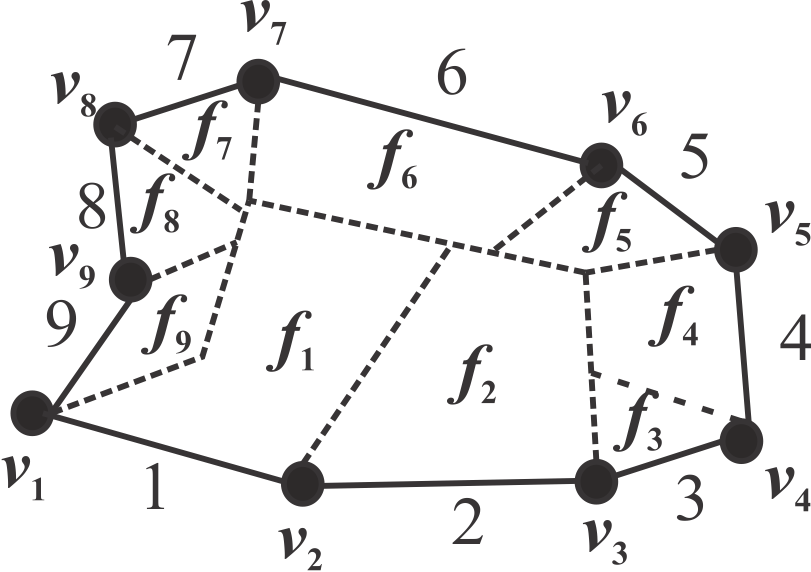
\includegraphics[width=.5\linewidth]{pic03.png}
  \caption{Possible solution.}
  \label{fig:sub2}
\end{subfigure}
\caption{Problem input/output representation.}
\label{fig:one}
\end{figure}
\FloatBarrier

Digital elevation model (DEM) can be used to automatically generate catchment areas. San Francisco Department of Public Work (SF DPW) has applied similar techniques at a fine resolution.  These results are used to study pipe hydraulics for San Francisco’s several systems. To automated the drainage catchment delineation process,  computer script in ArcGIS Model Builder called the Urbane Drainage Model is created. The Urbane Drainage Model is based on the commonly used “sleepiest path” approach,  using a gridded evaluation model, catchment areas were delineated for the City of San Francisco. A sub-catchment was created for each drain in the area.

The problem  mathematically is formulated in the following way:

A polygon $P$ is given by the Cartesian coordinates of its vertices (corresponding to Manholes) and its edges $i=1,..,N$. Each edge has a pipe with certain quantity of water which can drain. The polygon has $N$ edges. Total drain quantity of the polygon is denoted with $F$ and its value is 100\%. Each edge has a drain quantity of $f_i$, such as  $F = \sum f_i$.

For visualization purposes we look for a geometric partitioning of the polygon, such that the area of the $i$-th part is equal to $f_i$.

As example, for the given data in Fig. \ref{fig:sub3} and standard visual interpretation in Fig. \ref{fig:sub4}, possible visual (geometrical) interpretation is presented in Fig. \ref{fig:sub2}.

\begin{figure}[h!]
\centering
\begin{subfigure}{.5\textwidth}
  \centering
  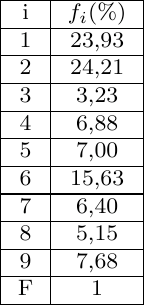
\includegraphics[width=.4\linewidth]{pic07.png}
  \caption{Table data.}
  \label{fig:sub3}
\end{subfigure}%
\begin{subfigure}{.5\textwidth}
  \centering
  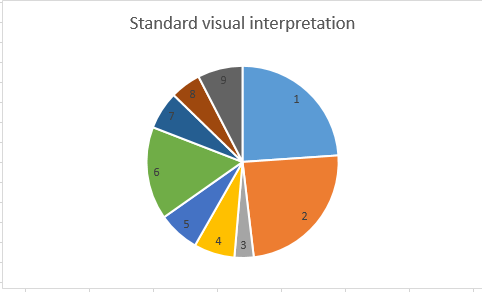
\includegraphics[width=.8\linewidth]{pic02.png}
  \caption{Pie chart.}
  \label{fig:sub4}
\end{subfigure}
\caption{Test case data.}
\label{fig:two}
\end{figure}
\FloatBarrier

\sect{2.~Solution approaches}

\subsect{2.1.~Numerical Evaluation of Solutions Quality}

For searching of empirical solutions it is convenient the polygon $P$ to be presented as grid of square pixels $p_{(x,y)}$. After transformation of the problem into 2D discrete space the quality of the solutions should be measured. A cost function with four components is selected. 

$$\min CF = B + W + A + D$$

As minimal is the cost function as better is the solution. The simplest const function model is the linear model ant that is why it was selected, but other variations are also possible and it will be interesting to be investigated in some further studies. 

$$B = \sum_{i=1}^N b_i$$

Where $b_i$ is the number of vertices of the sub-polygon $T_i$ attached to the edge $i$. The lowest value of $B$ is achieved when all sub-polygons are triangles and in this case $B$ has value of $N$. Upper of theoretical limit of $B$ is the total number of pixels which are part of the polygon $P$.

$$W= count( p_{(x,y)} ), p_{(x,y)} \notin T_i, \forall{ T_i}, i=1, \dots, N$$

The lower bound of $W$ is zero when there is no uncovered area in the polygon $P$. The upper bound of $W$ is the total number of pixels inside the polygon $P$. In this case any sub-area is covered. 

$$A = \sum_{(a_i - f_i)>0}(a_i - f_i)$$

Where $a_i$ is the percentage of the area which sub-polygon $T_i$ takes from the polygn $P$. The lowest value of $A$ is zero and it means that there is no overloading of any sub-area. Theoretical upper value of $A$ is one hundred and it can be achieved when all quantities $f_i$ are zero, but sub-polygons $T_i$ fulfill the polygon $P$.

$$D = \sum_{i=1}^N \frac{\sum_{j=1}^k d_{ij}}k$$

Where $d_{ij}$ is the distance between each pixel $j$ part of the sub-polygon $T_i$ and the edge $i$ of the polygon $P$. Also $k$ is the total number of pixels in the sub-polygon $T_i$. The lowest theoretical value of D is zero, but such solution is not acceptable, because it will mean that there is no sub-polygons (all $T_i$ polygons are with surface of zero). We are not going to provide estimation for the upper bound of D, because its calculation is complicated. 

\begin{figure}[h!]
\centering
\begin{subfigure}{.5\textwidth}
  \centering
  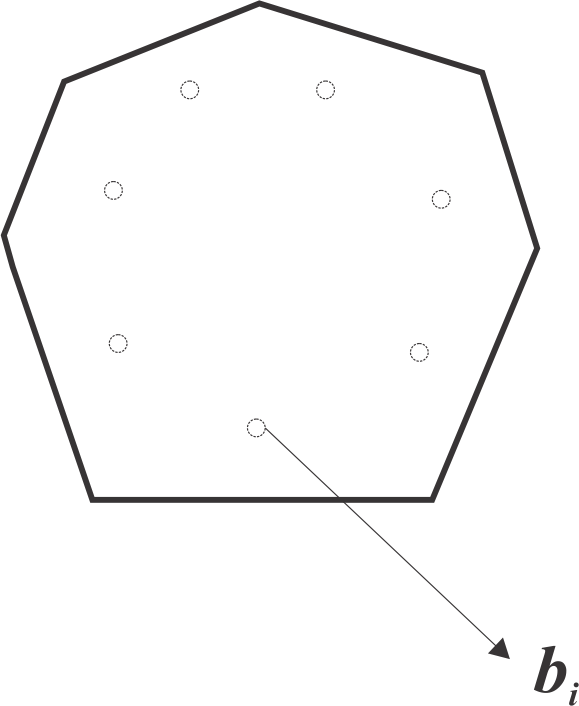
\includegraphics[width=.5\linewidth]{pic04.png}
  \caption{Point near to each polygon $P$ edge.}
  \label{fig:sub5}
\end{subfigure}%
\begin{subfigure}{.5\textwidth}
  \centering
  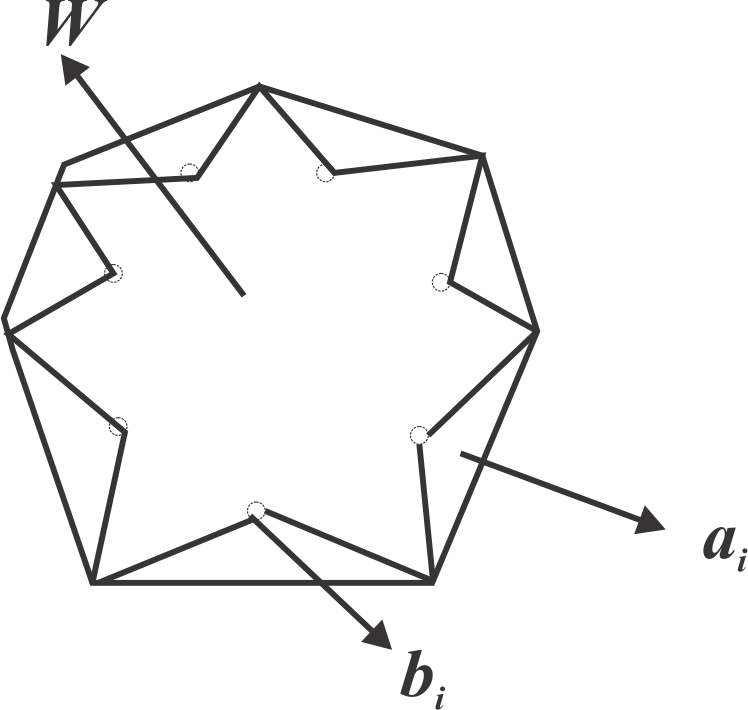
\includegraphics[width=.6\linewidth]{pic05.png}
  \caption{Polygon $P$ separation.}
  \label{fig:sub6}
\end{subfigure}
\caption{Sub-polygons $T_i$ related to each side of the polygon.}
\label{fig:three}
\end{figure}

\begin{figure}[h!]
  \centering
  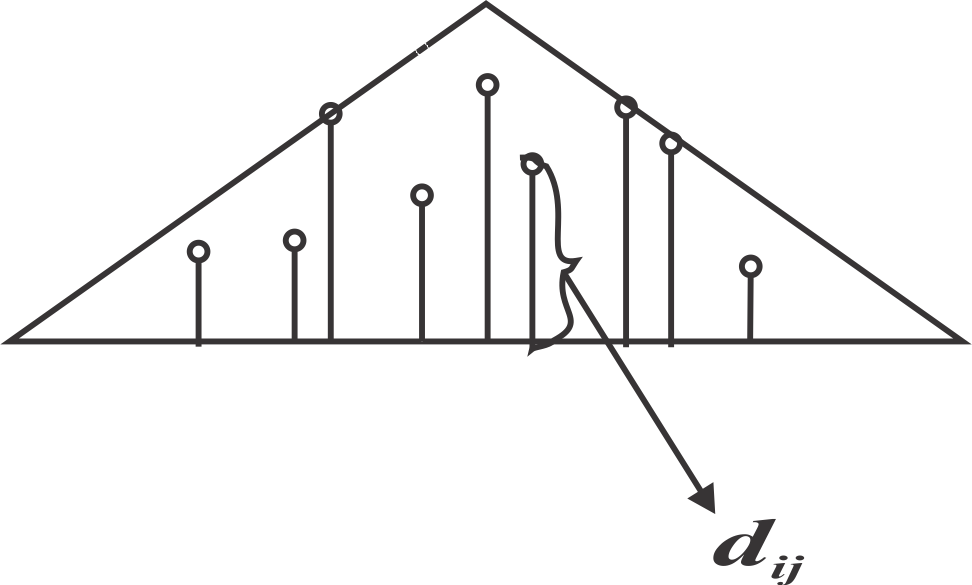
\includegraphics[width=.5\linewidth]{pic06.png}
  \caption{Average distance of all pixels in the sub-plygon $T_i$ to the polygon $P$ edge.}
\label{fig:four}
\end{figure}
\FloatBarrier

\subsect{2.2.~Monte Carlo Flooding Algorithm}

The idea for the algorithm comes from the real life natural floods. If we invert the process and instead of chatchmens we put liquid sources in the centers of the polygon $P$ edges, we can spill a liquid with certain quantities $f_i$. After that we can observe how the liquid will fulfill the polygon $P$ by imagine that all quantities $f_i$ are with different colors. The algorithm is in the group of the Monte Carlo algorithms, because virtual flooding process is based on random pixels selection ( the source code is available at http://github.com/TodorBalabanov/ESGI-132-Geometric-Visualization-of-a-Polygon-Area-Partitioning ). Pseudocode is as follows:

\newpage
\noindent\rule{\textwidth}{1pt}
\begin{itemize}
\item[Step 1] For $i = 1$ to $N$
\item[Step 2] Initialize $l$ with zero and flooded area $c_i^0$, as single pixel in the middle of the edge $i$.
	\begin{itemize}
	\item[Step 3] While ($c_i^l \leq f_j$)
		\begin{itemize}
		\item[Step 3.1] Select random pixel $t_{(x,y)}$ which belongs to $W$ area, but has direct neighbouring pixel which belongs to $c_i^l$,
		\item[Step 3.2] Add $t_{(x,y)}$ to $c_i^l$.
		\item[Step 3.3] Increase $l$.
		\end{itemize}
	\end{itemize}
\end{itemize}
\noindent\rule{\textwidth}{1pt}

The final result of the algorithm is $N$ irregular shapes.

\subsect{2.3.~Offsetting Polygon Algorithm}

The main idea of the offsetting polygon approach is to fill the initial polygon with smaller ones of which each side is parallel to the corresponding one of the initial polygon. The initial algorithm is the following:

\noindent\rule{\textwidth}{1pt}
\begin{itemize}

\item[Step 1.] Draw a parallel segment to each side of the polygon, creating a smaller polygon inside each with an offesetting distance $h$. 
\item[Step 2.] Connect each of the corresponding vertices of each polygon and calculate the area of the trapezoids created.
\item[Step 3.] Calculate the area of the created trapezoids and check if it fits the data.
\begin{itemize}
\item[Step 3.1] If the area doesn't fit we continue with creating parallel polygons.
\item[Step 3.2] If the desired area is accomplished, fix the side of the corresponding trapezoid and stop drawing parallel sides for it.
\end{itemize}
  \item[Step 4] Continue \textit{Step 2} until the data is fitted.
\end{itemize}
\noindent\rule{\textwidth}{1pt}

The initial algorithm applied worked very well for convex polygons. But when the algorithm was tested on a concave polygon the results were unsatisfying and this approach needed to be modified. The modifications were in the form of defining a different offsetting step $h$ for each side i.e. we will have $n$ different distances, where $n$ is the number of the polygon's sides. Following this approach, we end up with the concave angle's corresponding sides intersect with the opposite side. At this iteration of the algorithm, we modify the distance between the parallel sides so that they cross the opposite side at one point. As a result, we obtain two smaller polygons for which we apply the same algorithm. By the end with this modified approach we get a triangle(s) which area to side distributions can be found easily.

\sect{3.~Experimens and Results}

\subsect{3.1.~Monte Carlo Flooding Algorithm}

Monte Carlo Flooding is a very efficient heuristics, but it has a few disadvantages. At first place 2D space is divided on shapes similar to semi-circles when polygons are required. At second place it is obvious that distribution of the sub-areas is not optimal, which is clearly visible in Fig. \ref{fig:sub7}. This makes it inappropriate for acceptable solution of the problem, but very proper for initial idea of partitioning. 

\begin{figure}[h!]
\centering
\begin{subfigure}{.5\textwidth}
  \centering
  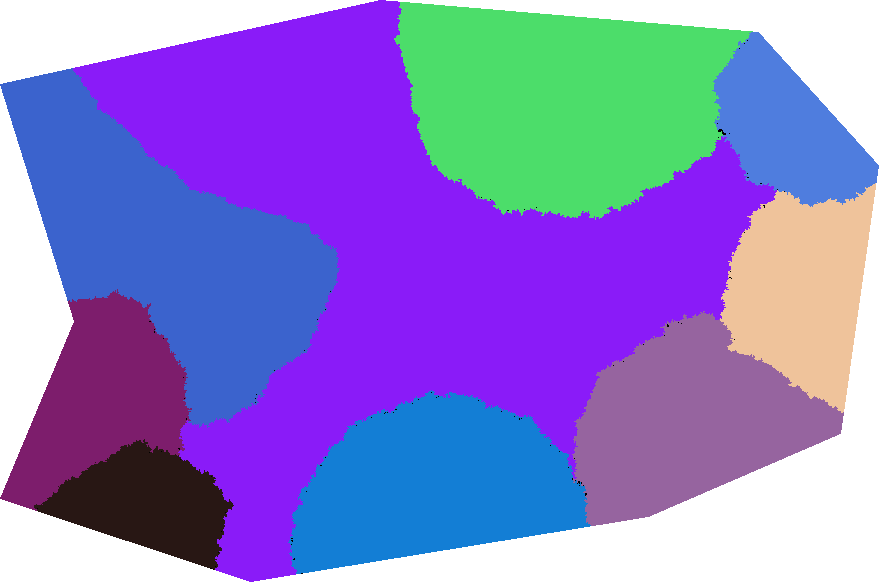
\includegraphics[width=.5\linewidth]{pic08.png}
  \caption{Test case 1.}
  \label{fig:sub7}
\end{subfigure}
\begin{subfigure}{.5\textwidth}
  \centering
  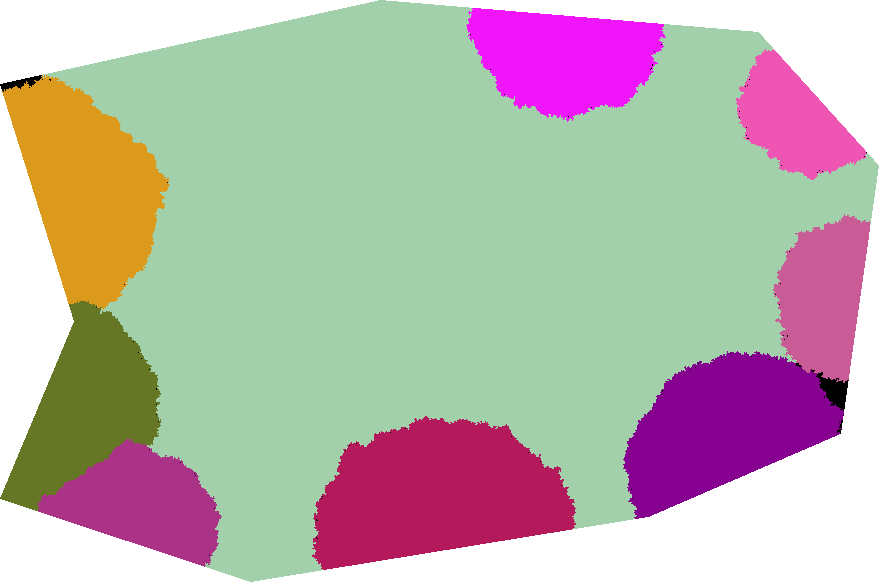
\includegraphics[width=.5\linewidth]{pic09.png}
  \caption{Test case 2.}
  \label{fig:sub8}
\end{subfigure}
\caption{Monte Carlo Flooding algorithm results.}
\label{fig:five}
\end{figure}
\FloatBarrier

\subsect{3.2.~Offsetting Polygon Algorithm}

Offsetting polygon method divides the polygon into smaller polygons with sides parallel to the initial one. Figure \ref{fig:sub11} shows the intitial step of the algorithm. Figure \ref{fig:sub12} is the result from the unmodified algorithm, ran on a concave polygon. Figure \ref{fig:sub13} contains the step with the intersecting parts of the polygon and a final result of two smaller triangles.

\begin{figure}[h!] 
\centering
\begin{subfigure}{.5\textwidth}
  \centering
  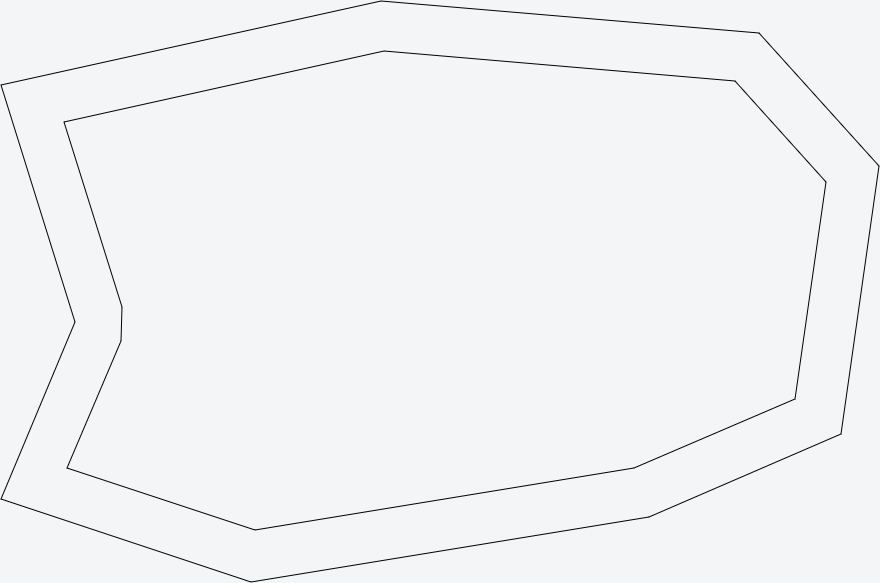
\includegraphics[width=.5\linewidth]{pic12.png}
  \caption{Initial step.}
  \label{fig:sub11}
\end{subfigure}
\begin{subfigure}{.5\textwidth}
  \centering
  
\includegraphics[width=.5\linewidth]{pic13.png}
  \caption{Final result.}
  \label{fig:sub12}
\end{subfigure}
\caption{Offsetting Polygon algorithm results.}
\label{fig:seven}
\end{figure}
\FloatBarrier

Figure 8 shows the interception step of the modified algorithm and Figure 9 shows the final result of the algorithm.

\begin{figure}[h!]
  \centering
  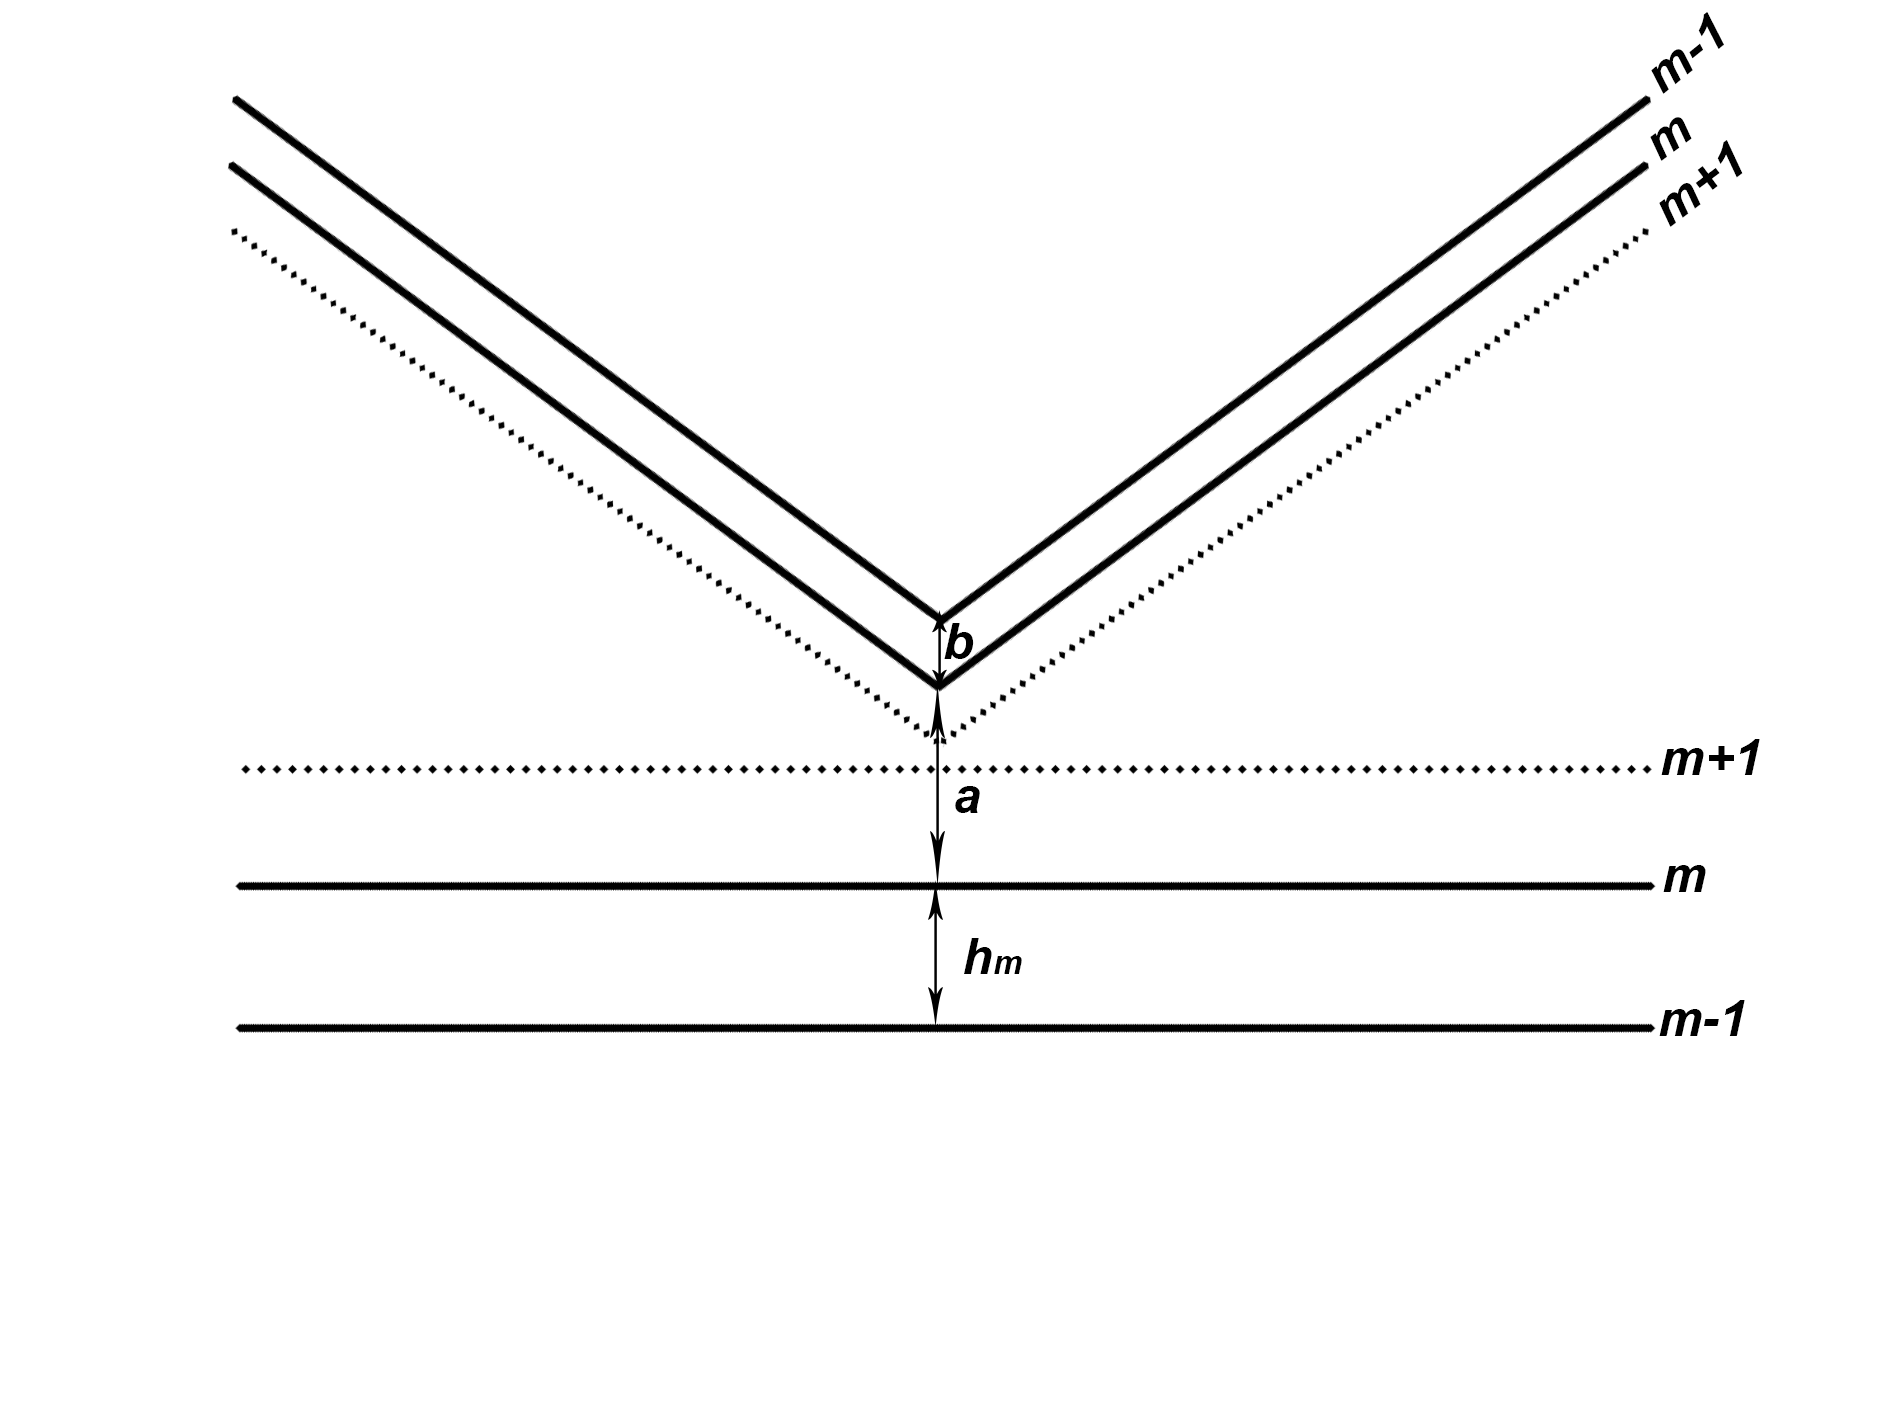
\includegraphics[width=.6\linewidth]{pic15.png}
  \caption{Intercepting part of the algorithm.}
\end{figure}
\FloatBarrier

\begin{figure}[h!]
  \centering
  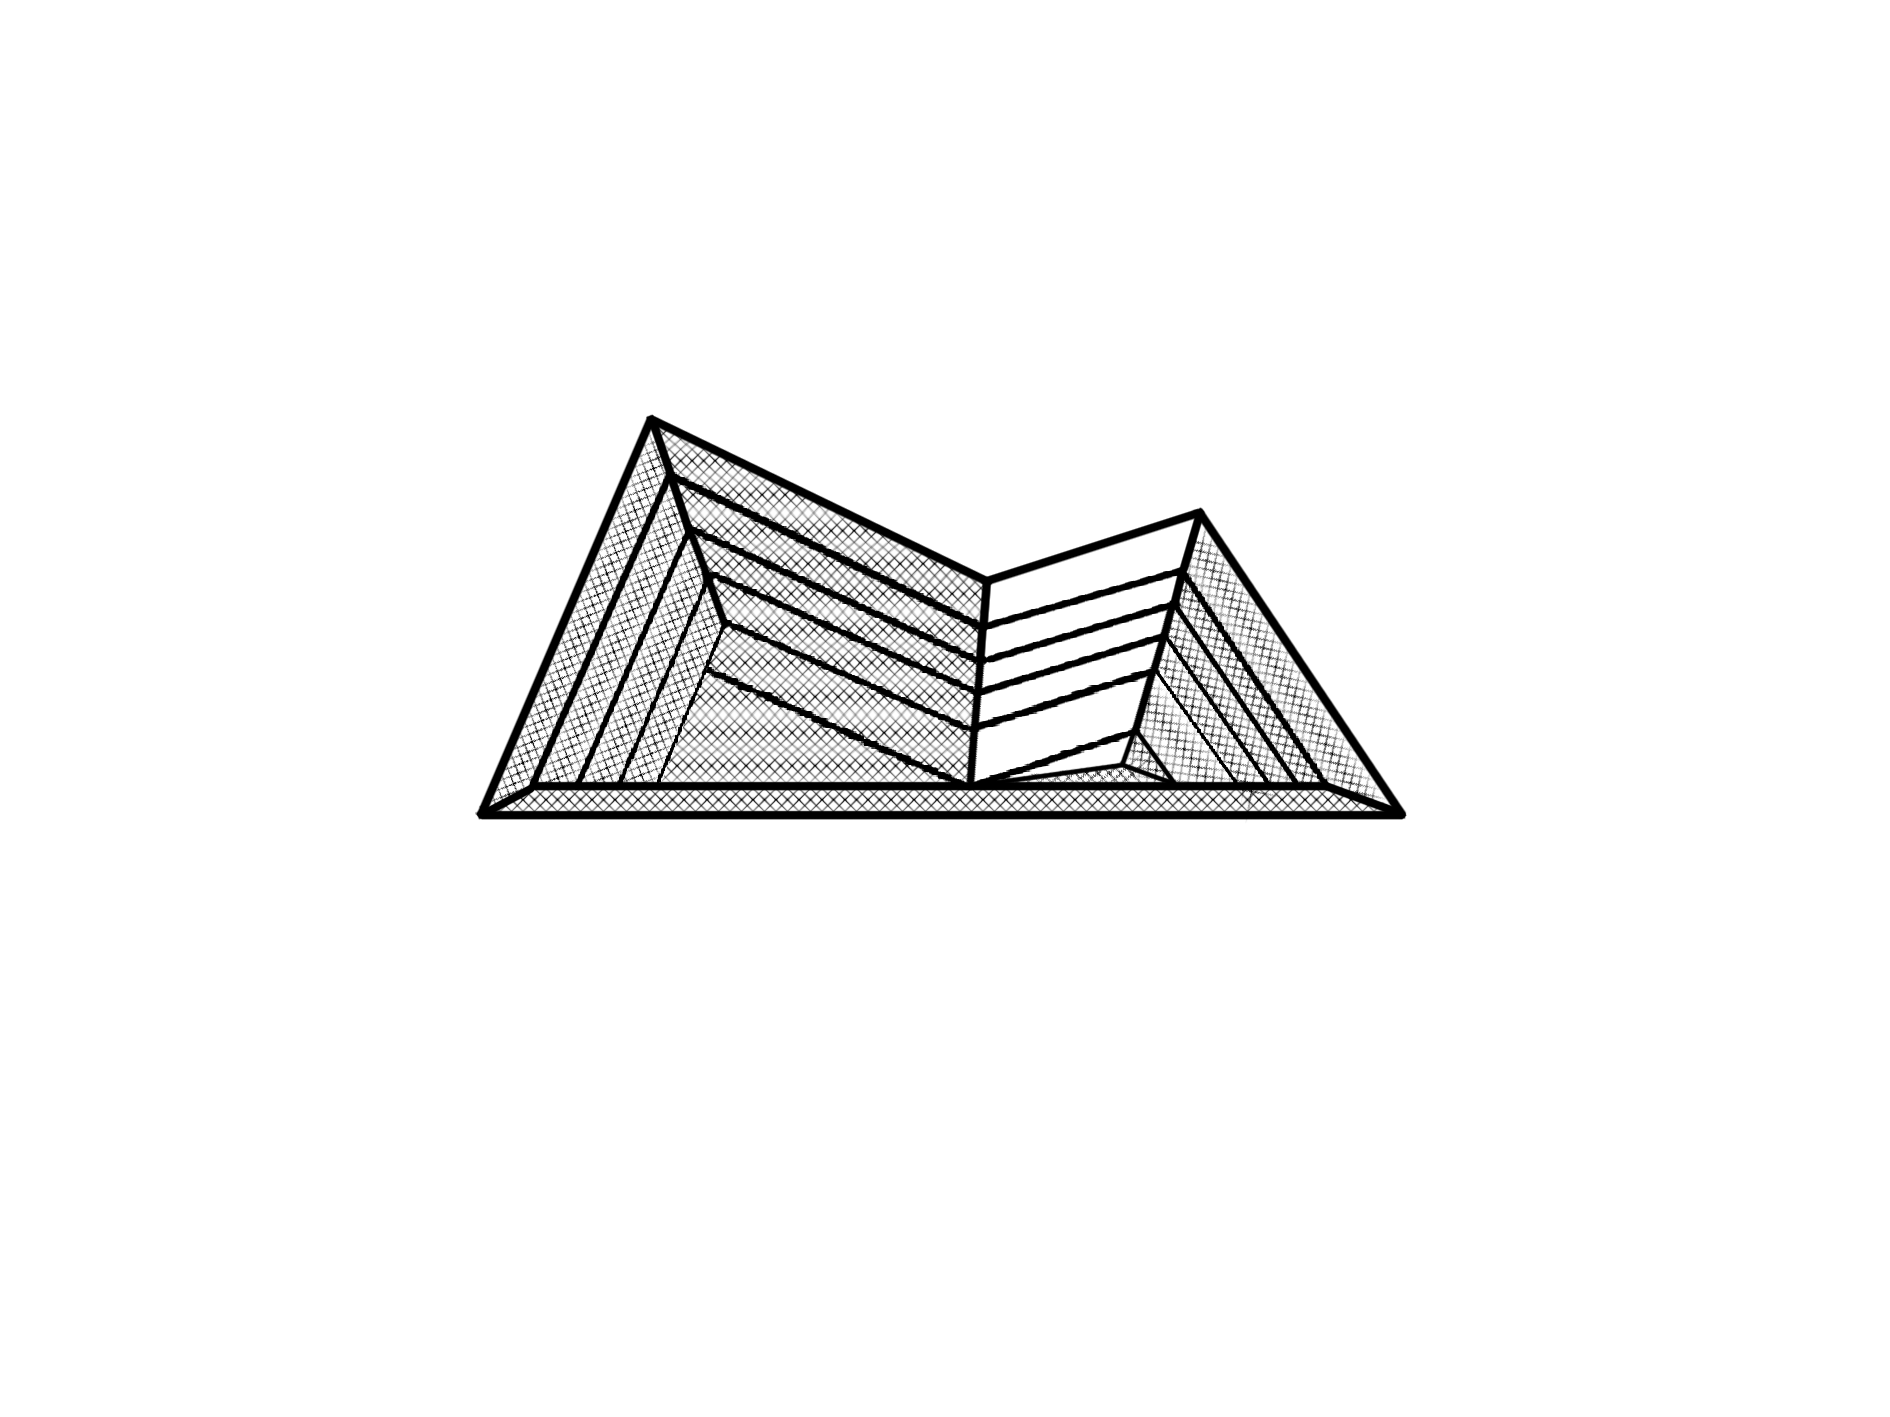
\includegraphics[width=.9\linewidth]{pic14.png}
  \caption{Modified offsetting polygon algorithm.}
\end{figure}
\FloatBarrier

\sect{Conclusions}

The experimental results show that the Offsetting Polygon algorithm can produce much better results than Monte Carlo Flooding algorithm. Monte Carlo Flooding algorithm is useful for initial idea of polygon separation.

\def\bibname{{\Large\bf References}}
\begin{thebibliography}{99}

\bibitem{han:bra:1} Han, D., and Bray, M. “Automated Thiessen polygon generation”, Water resources research, vol. 42, 2006.

\bibitem{mai:mik:1} Mair M., Mikovits C., Sengthaler M., Schoepf M., Kinzel H., Urich C., Kleidorfer M., Sitzenfrei R. and Rauch W, “The application of a Web-geographic information system for improving urban water cycle modelling “  Water Science and Technology 70(11), 2014, pp.1838-1846.

\bibitem{lay:day:1} Laycock R. G., Day A. M.”Automatically generating large urban environments based on the footprint data of buildings”, Proceedings of the eighth ACM symposium on Solid modeling and applications (New York, NY, USA), ACM Press, 2003, pp. 346–351.

\bibitem{lockie:1} Lockie T, “Catchment Modelling using SWMM” Modelling Stream at the 49th Water New Zealand Annual Conference and Expo, 2009.

\end{thebibliography}

\end{document}
